% answers.tex —— 2007 年·普通高等学校招生考试·新课标卷·文科 · 参考答案与详细解析片段
% 由 tools/generate_projects.py 依来源总账自 2007/2007_数学真题_新课标文_试题.md + 2007/2007_数学真题_新课标文_解析正文.md + 2007/2007_数学真题_新课标文_答案要点.md 生成，勿手改（改源 MD 后重跑）


\begin{gktip}
固定候选 PDF 仅含题面，无答案、解析和评分标准，原卷亦未标注分值；以下为非官方编者独立推导，官方答案字段为空。来源发布者、出版者、版次与官方身份均未核。
\end{gktip}

\begin{answer}
\gksolhead{1}{}

\textbf{题目}：

设集合 $A=\{x\mid x>-1\}$，$B=\{x\mid -2<x<2\}$，则 $A\cup B=$（　）

（A）$\{x\mid x>-2\}$

（B）$\{x\mid x>-1\}$

（C）$\{x\mid -2<x<-1\}$

（D）$\{x\mid -1<x<2\}$

\Needspace{4\baselineskip}
\textbf{解析}

\Needspace{5\baselineskip}
$A=\{x\mid x>-1\}=(-1,+\infty)$，$B=\{x\mid -2<x<2\}=(-2,2)$。并集取两区间的全部：

\nopagebreak[4]
\[A\cup B=(-2,+\infty)=\{x\mid x>-2\},\]

选 A。

（判断要点：并集是“至少属于一个集合”，$B$ 已经把 $-2$ 到 $-1$ 这一段包含进来，故左端点为 $-2$。）

\gkanswer{答案：A。}

\end{answer}
\begin{answer}
\gksolhead{2}{}

\textbf{题目}：

已知命题 $p$：$\forall x\in\mathbf R$，$\sin x\leqslant1$，则（　）

（A）$\neg p$：$\exists x\in\mathbf R$，$\sin x\geqslant1$

（B）$\neg p$：$\forall x\in\mathbf R$，$\sin x\geqslant1$

（C）$\neg p$：$\exists x\in\mathbf R$，$\sin x>1$

（D）$\neg p$：$\forall x\in\mathbf R$，$\sin x>1$

\Needspace{4\baselineskip}
\textbf{解析}

\Needspace{5\baselineskip}
全称命题的否定，先把全称量词改为存在量词，再否定结论：

\nopagebreak[4]
\[\neg p:\ \exists x\in\mathbf R,\ \sin x>1.\]

原结论 $\sin x\leqslant1$ 的否定是 $\sin x>1$，不是 $\geqslant1$。故选 C。

（判断要点：$\leqslant$ 的否定是 $>$，不是 $\geqslant$；量词也要由“任意”改为“存在”。）

\gkanswer{答案：C。}

\end{answer}
\begin{answer}
\gksolhead{3}{}

\textbf{题目}：

函数 $y=\sin\left(2x-\dfrac{\pi}{3}\right)$ 在区间 $\left[-\dfrac{\pi}{2},\pi\right]$ 的简图是（　）
\nopagebreak[4]
\begin{center}% 2007 年新课标卷文科第 3 题：函数 y=sin(2x-π/3) 在 [-π/2,π] 上的四个简图选项。
%   （A）为正确图象；（B）（C）（D）为相位不同的干扰项。
% 来源 PDF：gaokaomath-src/普通高考/2007/2007新课标文(海南,宁夏).pdf
% SHA-256：c8ee1632ac3a7a28aab1150f047a2e1c74398ca2944701e9165237897ae724e2
% 原页：2007新课标文(海南,宁夏).pdf 第 1 页（A3 三栏）第 1 栏，书页码 393。
% 重绘依据：按原页四个小图的零点、极值位置与坐标轴标注重绘；横轴以 π 为单位。
\begin{tikzpicture}[x=2.6cm, y=1.6cm, semithick,
  every node/.style={inner sep=1pt, font=\small}]

  % ================= （A）正确图象 =================
  \begin{scope}[shift={(0cm,0cm)}]
    \draw[->,>=stealth] (-0.66,0) -- (1.20,0) node[right] {$x$};
    \draw[->,>=stealth] (0,-1.22) -- (0,1.38) node[above] {$y$};
    \draw[domain=-0.5:1,samples=200,line width=1pt]
      plot (\x,{sin(deg(2*pi*\x - pi/3))});
    \draw[dashed] (-0.5,0) -- (-0.5,{sin(deg(-pi - pi/3))});
    \draw[dashed] (1,0) -- (1,{sin(deg(2*pi - pi/3))});
    \node[below] at (-0.5,0) {$-\frac{\pi}{2}$};
    \node[below left=1pt] at (0,0) {$O$};
    \node[below] at (1,0) {$\pi$};
    \node[left=2pt] at (0,1) {$1$};
    \node[left=2pt] at (0,-1) {$-1$};
    \node[below] at (0.55,-1.55) {（A）};
  \end{scope}

  % ================= （B） =================
  \begin{scope}[shift={(7.2cm,0cm)}]
    \draw[->,>=stealth] (-0.66,0) -- (1.20,0) node[right] {$x$};
    \draw[->,>=stealth] (0,-1.22) -- (0,1.38) node[above] {$y$};
    \draw[domain=-0.5:1,samples=200,line width=1pt]
      plot (\x,{sin(deg(2*pi*\x + pi/3))});
    \draw[dashed] (-0.5,0) -- (-0.5,{sin(deg(-pi + pi/3))});
    \draw[dashed] (1,0) -- (1,{sin(deg(2*pi + pi/3))});
    \node[below] at (-0.5,0) {$-\frac{\pi}{2}$};
    \node[below left=1pt] at (0,0) {$O$};
    \node[below] at (1,0) {$\pi$};
    \node[left=2pt] at (0,1) {$1$};
    \node[left=2pt] at (0,-1) {$-1$};
    \node[below] at (0.55,-1.55) {（B）};
  \end{scope}

  % ================= （C） =================
  \begin{scope}[shift={(0cm,-5.35cm)}]
    \draw[->,>=stealth] (-0.66,0) -- (1.20,0) node[right] {$x$};
    \draw[->,>=stealth] (0,-1.22) -- (0,1.38) node[above] {$y$};
    \draw[domain=-0.5:1,samples=200,line width=1pt]
      plot (\x,{sin(deg(2*pi*\x - 2*pi/3))});
    \draw[dashed] (-0.5,0) -- (-0.5,{sin(deg(-pi - 2*pi/3))});
    \draw[dashed] (1,0) -- (1,{sin(deg(2*pi - 2*pi/3))});
    \node[below] at (-0.5,0) {$-\frac{\pi}{2}$};
    \node[below left=1pt] at (0,0) {$O$};
    \node[below] at (1,0) {$\pi$};
    \node[left=2pt] at (0,1) {$1$};
    \node[left=2pt] at (0,-1) {$-1$};
    \node[below] at (0.55,-1.55) {（C）};
  \end{scope}

  % ================= （D） =================
  \begin{scope}[shift={(7.2cm,-5.35cm)}]
    \draw[->,>=stealth] (-0.66,0) -- (1.20,0) node[right] {$x$};
    \draw[->,>=stealth] (0,-1.22) -- (0,1.38) node[above] {$y$};
    \draw[domain=-0.5:1,samples=200,line width=1pt]
      plot (\x,{sin(deg(2*pi*\x + 2*pi/3))});
    \draw[dashed] (-0.5,0) -- (-0.5,{sin(deg(-pi + 2*pi/3))});
    \draw[dashed] (1,0) -- (1,{sin(deg(2*pi + 2*pi/3))});
    \node[below] at (-0.5,0) {$-\frac{\pi}{2}$};
    \node[below left=1pt] at (0,0) {$O$};
    \node[below] at (1,0) {$\pi$};
    \node[left=2pt] at (0,1) {$1$};
    \node[left=2pt] at (0,-1) {$-1$};
    \node[below] at (0.55,-1.55) {（D）};
  \end{scope}
\end{tikzpicture}
\end{center}
\nopagebreak[4]
\Needspace{4\baselineskip}
\textbf{解析}

\Needspace{5\baselineskip}
令 $y=0$：

\nopagebreak[4]
\[2x-\frac{\pi}{3}=k\pi\ \Rightarrow\ x=\frac{\pi}{6}+\frac{k\pi}{2}.\]

\Needspace{5\baselineskip}
在 $\left[-\dfrac{\pi}{2},\pi\right]$ 内取 $k=-1,0,1,2$，得零点

\nopagebreak[4]
\[-\frac{\pi}{3},\quad \frac{\pi}{6},\quad \frac{2\pi}{3},\quad \frac{7\pi}{6}.\]

\Needspace{5\baselineskip}
其中 $\dfrac{7\pi}{6}>\pi$，舍去。再取特殊点：

\nopagebreak[4]
\[x=-\frac{\pi}{2}:\ y=\sin\left(-\pi-\frac{\pi}{3}\right)=\frac{\sqrt3}{2}>0,\]

\nopagebreak[4]
\[x=0:\ y=\sin\left(-\frac{\pi}{3}\right)=-\frac{\sqrt3}{2}<0,\]

\nopagebreak[4]
\[x=\pi:\ y=\sin\left(2\pi-\frac{\pi}{3}\right)=-\frac{\sqrt3}{2}<0.\]

图象应在 $-\dfrac{\pi}{2}$ 处为正、经过 $-\dfrac{\pi}{3}$ 变号、在 $x=-\dfrac{\pi}{12}$ 附近取最小值、经过 $\dfrac{\pi}{6}$ 上升、在 $x=\dfrac{5\pi}{12}$ 附近取最大值、经过 $\dfrac{2\pi}{3}$ 后下降。与四图比对，只有（A）符合。选 A。

（判断要点：先解出区间内全部零点，再用 $x=0$ 与端点的符号定位；最大值横坐标 $\dfrac{5\pi}{12}$ 在 $\dfrac{\pi}{6}$ 与 $\dfrac{\pi}{2}$ 之间。）

\gkanswer{答案：A。}

\end{answer}
\begin{answer}
\gksolhead{4}{}

\textbf{题目}：

已知平面向量 $\boldsymbol a=(1,1)$，$\boldsymbol b=(1,-1)$，则向量 $\dfrac12\boldsymbol a-\dfrac32\boldsymbol b=$（　）

（A）$(-2,-1)$

（B）$(-2,1)$

（C）$(-1,0)$

（D）$(-1,2)$

\Needspace{4\baselineskip}
\textbf{解析}

\nopagebreak[4]
\[\frac12\boldsymbol a=\left(\frac12,\frac12\right),\qquad \frac32\boldsymbol b=\left(\frac32,-\frac32\right).\]

\Needspace{5\baselineskip}
相减：

\nopagebreak[4]
\[\frac12\boldsymbol a-\frac32\boldsymbol b=\left(\frac12-\frac32,\frac12+\frac32\right)=(-1,2),\]

选 D。

（判断要点：$\boldsymbol b=(1,-1)$ 乘 $\dfrac32$ 后第二分量是 $-\dfrac32$，作差时负负得正。）

\gkanswer{答案：D。}

\end{answer}
\begin{answer}
\gksolhead{5}{}

\textbf{题目}：

如果执行下面的程序框图，那么输出的 $S=$（　）
\nopagebreak[4]
\begin{center}% 2007 年新课标卷文科第 5 题：程序框图（k 从 1 到 50 累加 2k）。
% 来源 PDF：gaokaomath-src/普通高考/2007/2007新课标文(海南,宁夏).pdf
% SHA-256：c8ee1632ac3a7a28aab1150f047a2e1c74398ca2944701e9165237897ae724e2
% 原页：2007新课标文(海南,宁夏).pdf 第 1 页（A3 三栏）第 1 栏，书页码 393。
% 重绘依据：按原页流程与分支方向重绘；循环体为 S=S+2k、k=k+1。
\begin{tikzpicture}[scale=1.0, semithick,
  every node/.style={inner sep=2pt},
  box/.style={draw, rounded corners=2pt, minimum width=1.9cm,
    minimum height=0.55cm, align=center},
  para/.style={draw, trapezium, trapezium left angle=70,
    trapezium right angle=110, minimum width=2.4cm, minimum height=0.55cm,
    align=center},
  dec/.style={draw, diamond, aspect=2.4, minimum width=2.8cm,
    minimum height=1.1cm, align=center},
  arr/.style={->, >=stealth}]

  \node[box]  (start) at (0,7.2) {开始};
  \node[box]  (init)  at (0,6.3) {$k=1$};
  \node[box]  (sum)   at (0,5.4) {$S=0$};
  \node[dec]  (test)  at (0,4.2) {$k\leqslant50$?};
  \node[box]  (add)   at (0,2.95) {$S=S+2k$};
  \node[box]  (inc)   at (0,2.15) {$k=k+1$};
  \node[para] (out)   at (4.6,4.2) {输出 $S$};
  \node[box]  (end)   at (4.6,3.3) {结束};

  \draw[arr] (start) -- (init);
  \draw[arr] (init) -- (sum);
  \draw[arr] (sum) -- (test);
  \draw[arr] (test.south) -- node[left] {是} (add.north);
  \draw[arr] (add) -- (inc);
  \draw[arr] (inc.west) -- (-2.5,2.15) -- (-2.5,4.75) -- (0,4.75);
  \draw[arr] (test.east) -- node[above] {否} (out.west);
  \draw[arr] (out) -- (end);
\end{tikzpicture}
\end{center}
\nopagebreak[4]
（A）$2450$

（B）$2500$

（C）$2550$

（D）$2652$

\Needspace{4\baselineskip}
\textbf{解析}

\Needspace{5\baselineskip}
循环从 $k=1$ 开始，每次判断 $k\leqslant50$，成立则执行

\nopagebreak[4]
\[S=S+2k,\qquad k=k+1.\]

\Needspace{5\baselineskip}
故累加 $2\times1,2\times2,\cdots,2\times50$：

\nopagebreak[4]
\[S=2(1+2+\cdots+50)=2\times\frac{50\times51}{2}=2550,\]

选 C。

（判断要点：循环共 $50$ 项；$1+2+\cdots+50=1275$，乘 $2$ 得 $2550$。）

\gkanswer{答案：C。}

\end{answer}
\begin{answer}
\gksolhead{6}{}

\textbf{题目}：

已知 $a$，$b$，$c$，$d$ 成等比数列，且曲线 $y=x^2-2x+3$ 的顶点是 $(b,c)$，则 $ad$ 等于（　）

（A）$3$

（B）$2$

（C）$1$

（D）$-2$

\Needspace{4\baselineskip}
\textbf{解析}

\Needspace{5\baselineskip}
配方：

\nopagebreak[4]
\[y=x^2-2x+3=(x-1)^2+2,\]

\Needspace{5\baselineskip}
顶点为 $(1,2)$，故

\nopagebreak[4]
\[b=1,\qquad c=2.\]

\Needspace{5\baselineskip}
$a$，$b$，$c$，$d$ 成等比数列，即 $a,1,2,d$ 成等比，公比

\nopagebreak[4]
\[q=\frac21=2.\]

\Needspace{5\baselineskip}
故

\nopagebreak[4]
\[a=\frac{1}{2},\qquad d=2\times2=4,\]

\nopagebreak[4]
\[ad=\frac12\times4=2,\]

选 B。

（判断要点：顶点横坐标是 $-\dfrac{-2}{2}=1$，纵坐标代回得 $2$；等比数列中 $b^2=ac$，也可先求 $a$。）

\gkanswer{答案：B。}

\end{answer}
\begin{answer}
\gksolhead{7}{}

\textbf{题目}：

已知抛物线 $y^2=2px$（$p>0$）的焦点为 $F$，点 $P_1(x_1,y_1)$，$P_2(x_2,y_2)$，$P_3(x_3,y_3)$ 在抛物线上，且 $2x_2=x_1+x_3$，则有（　）

（A）$|FP_1|+|FP_2|=|FP_3|$

（B）$|FP_1|^2+|FP_2|^2=|FP_3|^2$

（C）$2|FP_2|=|FP_1|+|FP_3|$

（D）$|FP_2|^2=|FP_1|\cdot|FP_3|$

\Needspace{4\baselineskip}
\textbf{解析}

\Needspace{5\baselineskip}
抛物线焦半径公式：

\nopagebreak[4]
\[|FP|=x+\frac p2.\]

\Needspace{5\baselineskip}
由 $2x_2=x_1+x_3$，两边加 $p$：

\nopagebreak[4]
\[2x_2+p=x_1+x_3+p,\]

\Needspace{5\baselineskip}
即

\nopagebreak[4]
\[2\left(x_2+\frac p2\right)=\left(x_1+\frac p2\right)+\left(x_3+\frac p2\right).\]

\Needspace{5\baselineskip}
故

\nopagebreak[4]
\[2|FP_2|=|FP_1|+|FP_3|,\]

选 C。

（判断要点：抛物线上的点到焦点距离等于 $x+\dfrac p2$；横坐标的等差关系加 $p$ 后仍成立。）

\gkanswer{答案：C。}

\end{answer}
\begin{answer}
\gksolhead{8}{}

\textbf{题目}：

已知某个几何体的三视图如下，根据图中标出的尺寸（单位：$\mathrm{cm}$），可得这个几何体的体积是（　）
\nopagebreak[4]
\begin{center}% 2007 年新课标卷文科第 8 题：三视图（正视图、侧视图、俯视图）及尺寸。
%   正视图为直角边 20、20 的直角三角形；侧视图为底边 20、高 20 的等腰三角形；
%   俯视图为 20×20 正方形并画对角线，右侧标注 10 与 10。
% 来源 PDF：gaokaomath-src/普通高考/2007/2007新课标文(海南,宁夏).pdf
% SHA-256：c8ee1632ac3a7a28aab1150f047a2e1c74398ca2944701e9165237897ae724e2
% 原页：2007新课标文(海南,宁夏).pdf 第 1 页（A3 三栏）第 2 栏，书页码 393。
% 重绘依据：按原页三个视图的位置、形状与尺寸标注重绘，单位 cm。
\begin{tikzpicture}[x=0.115cm, y=0.095cm, semithick,
  every node/.style={inner sep=1.5pt, font=\small}]

  % ---------------- 正视图 ----------------
  \begin{scope}[shift={(0cm,0cm)}]
    \draw (0,0) -- (20,0) -- (20,20) -- cycle;
    % 尺寸 20（下）
    \draw[<->,>=stealth] (0,-4) -- (20,-4);
    \draw (0,-1.5) -- (0,-5.5);
    \draw (20,-1.5) -- (20,-5.5);
    \node[below] at (10,-4) {$20$};
    % 尺寸 20（右）
    \draw[<->,>=stealth] (24,0) -- (24,20);
    \draw (22,0) -- (26,0);
    \draw (22,20) -- (26,20);
    \node[right] at (24,10) {$20$};
    \node[below] at (10,-9) {正视图};
  \end{scope}

  % ---------------- 侧视图 ----------------
  \begin{scope}[shift={(3.6cm,0cm)}]
    \draw (0,0) -- (20,0) -- (10,20) -- cycle;
    \draw[<->,>=stealth] (0,-4) -- (20,-4);
    \draw (0,-1.5) -- (0,-5.5);
    \draw (20,-1.5) -- (20,-5.5);
    \node[below] at (10,-4) {$20$};
    \node[below] at (10,-9) {侧视图};
  \end{scope}

  % ---------------- 俯视图 ----------------
  \begin{scope}[shift={(0.9cm,-3.6cm)}]
    \draw (0,0) rectangle (20,20);
    \draw (0,0) -- (20,20);
    \draw (0,20) -- (20,0);
    % 尺寸 20（下）
    \draw[<->,>=stealth] (0,-4) -- (20,-4);
    \draw (0,-1.5) -- (0,-5.5);
    \draw (20,-1.5) -- (20,-5.5);
    \node[below] at (10,-4) {$20$};
    % 右侧 10 与 10
    \draw[<->,>=stealth] (24,0) -- (24,10);
    \draw[<->,>=stealth] (24,10) -- (24,20);
    \draw (22,0) -- (26,0);
    \draw (22,10) -- (26,10);
    \draw (22,20) -- (26,20);
    \node[right] at (24,5) {$10$};
    \node[right] at (24,15) {$10$};
    \node[below] at (10,-9) {俯视图};
  \end{scope}
\end{tikzpicture}
\end{center}
\nopagebreak[4]
（A）$\dfrac{4000}{3}\ \mathrm{cm^3}$

（B）$\dfrac{8000}{3}\ \mathrm{cm^3}$

（C）$2000\ \mathrm{cm^3}$

（D）$4000\ \mathrm{cm^3}$

\Needspace{4\baselineskip}
\textbf{解析}

\Needspace{5\baselineskip}
三视图对应底面为 $20\times20$ 正方形、高为 $20$ 的四棱锥。体积

\nopagebreak[4]
\[V=\frac13\times20^2\times20=\frac{8000}{3}\ \mathrm{cm^3},\]

选 B。

（判断要点：三视图给出底面边长 $20$、高 $20$；四棱锥体积有 $\dfrac13$，不要漏。）

\gkanswer{答案：B。}

\end{answer}
\begin{answer}
\gksolhead{9}{}

\textbf{题目}：

若 $\dfrac{\cos2\alpha}{\sin\left(\alpha-\dfrac{\pi}{4}\right)}=-\dfrac{\sqrt2}{2}$，则 $\cos\alpha+\sin\alpha$ 的值为（　）

（A）$-\dfrac{\sqrt7}{2}$

（B）$-\dfrac12$

（C）$\dfrac12$

（D）$\dfrac{\sqrt7}{2}$

\Needspace{4\baselineskip}
\textbf{解析}

\nopagebreak[4]
\[\sin\left(\alpha-\frac{\pi}{4}\right)=\frac{\sin\alpha-\cos\alpha}{\sqrt2},\]

\nopagebreak[4]
\[\cos2\alpha=(\cos\alpha-\sin\alpha)(\cos\alpha+\sin\alpha).\]

\Needspace{5\baselineskip}
代入原式：

\nopagebreak[4]
\[\frac{(\cos\alpha-\sin\alpha)(\cos\alpha+\sin\alpha)}{\frac1{\sqrt2}(\sin\alpha-\cos\alpha)}=-\sqrt2(\cos\alpha+\sin\alpha).\]

\Needspace{5\baselineskip}
由已知等于 $-\dfrac{\sqrt2}{2}$，故

\nopagebreak[4]
\[\cos\alpha+\sin\alpha=\frac12,\]

选 C。

（判断要点：$\cos2\alpha$ 分解后与分母约去，只剩一个负号；不要漏掉 $\sqrt2$。）

\gkanswer{答案：C。}

\end{answer}
\begin{answer}
\gksolhead{10}{}

\textbf{题目}：

曲线 $y=\mathrm e^x$ 在点 $(2,\mathrm e^2)$ 处的切线与坐标轴所围三角形的面积为（　）

（A）$\dfrac94\mathrm e^2$

（B）$2\mathrm e^2$

（C）$\mathrm e^2$

（D）$\dfrac{\mathrm e^2}{2}$

\Needspace{4\baselineskip}
\textbf{解析}

\nopagebreak[4]
\[y=\mathrm e^x,\qquad y'=\mathrm e^x.\]

\Needspace{5\baselineskip}
在 $x=2$ 处，$y=\mathrm e^2$，斜率 $k=\mathrm e^2$。切线：

\nopagebreak[4]
\[y-\mathrm e^2=\mathrm e^2(x-2),\]

\Needspace{5\baselineskip}
即

\nopagebreak[4]
\[y=\mathrm e^2x-\mathrm e^2.\]

\Needspace{5\baselineskip}
令 $y=0$ 得 $x=1$；令 $x=0$ 得 $y=-\mathrm e^2$。三角形两直角边长为 $1$ 与 $\mathrm e^2$，面积

\nopagebreak[4]
\[S=\frac12\times1\times\mathrm e^2=\frac{\mathrm e^2}{2},\]

选 D。

（判断要点：切线与 $x$ 轴交于 $(1,0)$，不是 $(2,0)$；面积取截距长度乘积的一半。）

\gkanswer{答案：D。}

\end{answer}
\begin{answer}
\gksolhead{11}{}

\textbf{题目}：

已知三棱锥 $S-ABC$ 的各顶点都在一个半径为 $r$ 的球面上，球心 $O$ 在 $AB$ 上，$SO\perp$ 底面 $ABC$，$AC=\sqrt2r$，则球的体积与三棱锥体积之比是（　）

（A）$\pi$

（B）$2\pi$

（C）$3\pi$

（D）$4\pi$

\Needspace{4\baselineskip}
\textbf{解析}

\Needspace{5\baselineskip}
球心 $O$ 在 $AB$ 上，且 $A$、$B$ 在球面上，故 $AB$ 为球的直径：

\nopagebreak[4]
\[AB=2r.\]

又 $SO\perp$ 底面，$SO=r$。

\Needspace{5\baselineskip}
在 $\triangle ABC$ 中，$AB$ 为直径，由直径所对的圆周角为直角，得

\nopagebreak[4]
\[\angle ACB=90^\circ.\]

\Needspace{5\baselineskip}
已知 $AC=\sqrt2r$，故

\nopagebreak[4]
\[BC=\sqrt{AB^2-AC^2}=\sqrt{4r^2-2r^2}=\sqrt2r.\]

\Needspace{5\baselineskip}
底面面积

\nopagebreak[4]
\[S_{\triangle ABC}=\frac12\cdot AC\cdot BC=\frac12\cdot\sqrt2r\cdot\sqrt2r=r^2.\]

\Needspace{5\baselineskip}
三棱锥体积

\nopagebreak[4]
\[V_1=\frac13S_{\triangle ABC}\cdot SO=\frac13\cdot r^2\cdot r=\frac{r^3}{3}.\]

\Needspace{5\baselineskip}
球体积

\nopagebreak[4]
\[V_2=\frac43\pi r^3.\]

\Needspace{5\baselineskip}
故

\nopagebreak[4]
\[\frac{V_2}{V_1}=\frac{\frac43\pi r^3}{\frac{r^3}{3}}=4\pi,\]

选 D。

（判断要点：球心在弦 $AB$ 上说明 $AB$ 是直径；$SO$ 是高，长度为半径 $r$；底面是等腰直角三角形。）

\gkanswer{答案：D。}

\end{answer}
\begin{answer}
\gksolhead{12}{}

\textbf{题目}：

甲、乙、丙三名射箭运动员在某次测试中各射箭 $20$ 次，三人的测试成绩如下表

\begin{center}
\begin{tabular}{llllll}
\toprule
运动员 & 环数 & $7$ & $8$ & $9$ & $10$ \\
\midrule
甲 & 频数 & $5$ & $5$ & $5$ & $5$ \\
乙 & 频数 & $6$ & $4$ & $4$ & $6$ \\
丙 & 频数 & $4$ & $6$ & $6$ & $4$ \\
\bottomrule
\end{tabular}
\end{center}

$s_1$，$s_2$，$s_3$ 分别表示甲、乙、丙三名运动员这次测试成绩的标准差，则有（　）

（A）$s_3>s_1>s_2$

（B）$s_2>s_1>s_3$

（C）$s_1>s_2>s_3$

（D）$s_2>s_3>s_1$

\Needspace{4\baselineskip}
\textbf{解析}

\Needspace{5\baselineskip}
三人的平均成绩都是

\nopagebreak[4]
\[\bar x=\frac{7+8+9+10}{4}=8.5.\]

\Needspace{5\baselineskip}
方差分别为

\nopagebreak[4]
\[s_1^2=\frac{4\times(1.5)^2}{4}=1.25,\]

\nopagebreak[4]
\[s_2^2=\frac{6(1.5)^2+4(0.5)^2+4(0.5)^2+6(1.5)^2}{20}=1.45,\]

\nopagebreak[4]
\[s_3^2=\frac{4(1.5)^2+6(0.5)^2+6(0.5)^2+4(1.5)^2}{20}=1.05.\]

\Needspace{5\baselineskip}
故

\nopagebreak[4]
\[s_2>s_1>s_3,\]

选 B。

（判断要点：平均数相同，只比方差；乙在两端人数最多、丙在中间人数最多，故乙最分散、丙最集中。）

\gkanswer{答案：B。}

\end{answer}
\begin{answer}
\gksolhead{13}{}

\textbf{题目}：

已知双曲线的顶点到渐近线的距离为 $2$，焦点到渐近线的距离为 $6$，则该双曲线的离心率为\gkblank{}。

\Needspace{4\baselineskip}
\textbf{解析}

\Needspace{5\baselineskip}
设双曲线为

\nopagebreak[4]
\[\frac{x^2}{a^2}-\frac{y^2}{b^2}=1,\]

\Needspace{5\baselineskip}
渐近线 $bx-ay=0$。顶点 $(a,0)$ 到渐近线距离

\nopagebreak[4]
\[\frac{ab}{c}=2,\]

\Needspace{5\baselineskip}
焦点 $(c,0)$ 到渐近线距离

\nopagebreak[4]
\[b=6.\]

\Needspace{5\baselineskip}
由 $b=6$ 与 $\dfrac{ab}{c}=2$ 得

\nopagebreak[4]
\[\frac{6a}{c}=2\ \Rightarrow\ c=3a,\]

\Needspace{5\baselineskip}
故

\nopagebreak[4]
\[e=\frac ca=3.\]

（判断要点：焦点到渐近线的距离恒为 $b$；顶点到渐近线距离为 $\dfrac{ab}{c}$。）

\gkanswer{答案：$3$。}

\end{answer}
\begin{answer}
\gksolhead{14}{}

\textbf{题目}：

设函数 $f(x)=(x+1)(x+a)$ 为偶函数，则 $a=$\gkblank{}。

\Needspace{4\baselineskip}
\textbf{解析}

\Needspace{5\baselineskip}
展开：

\nopagebreak[4]
\[f(x)=(x+1)(x+a)=x^2+(a+1)x+a.\]

\Needspace{5\baselineskip}
二次函数为偶函数，其一次项必须为零：

\nopagebreak[4]
\[a+1=0\ \Rightarrow\ a=-1.\]

此时 $f(x)=x^2-1$，满足 $f(-x)=f(x)$。

（判断要点：多项式为偶函数当且仅当所有奇次项系数为零；这里只需看一次项。）

\gkanswer{答案：$-1$。}

\end{answer}
\begin{answer}
\gksolhead{15}{}

\textbf{题目}：

$\mathrm i$ 是虚数单位，$\mathrm i+2\mathrm i^2+3\mathrm i^3+\cdots+8\mathrm i^8=$\gkblank{}。（用 $a+b\mathrm i$ 的形式表示，$a$，$b\in\mathbf R$）

\Needspace{4\baselineskip}
\textbf{解析}

\Needspace{5\baselineskip}
利用 $\mathrm i$ 的幂的周期性：

\nopagebreak[4]
\[\mathrm i^1=\mathrm i,\quad \mathrm i^2=-1,\quad \mathrm i^3=-\mathrm i,\quad \mathrm i^4=1.\]

\Needspace{5\baselineskip}
逐项计算：

\nopagebreak[4]
\[\mathrm i+2\mathrm i^2+3\mathrm i^3+4\mathrm i^4=\mathrm i-2-3\mathrm i+4=2-2\mathrm i,\]

\nopagebreak[4]
\[5\mathrm i^5+6\mathrm i^6+7\mathrm i^7+8\mathrm i^8=5\mathrm i-6-7\mathrm i+8=2-2\mathrm i.\]

\Needspace{5\baselineskip}
相加：

\nopagebreak[4]
\[(2-2\mathrm i)+(2-2\mathrm i)=4-4\mathrm i.\]

（判断要点：每四项一轮回；实部为偶数项贡献，虚部为奇数项贡献，注意 $\mathrm i^3=-\mathrm i$。）

\gkanswer{答案：$4-4\mathrm i$。}

\end{answer}
\begin{answer}
\gksolhead{16}{}

\textbf{题目}：

已知 $\{a_n\}$ 是等差数列，$a_4+a_6=6$，其前 $5$ 项和 $S_5=10$，则其公差 $d=$\gkblank{}。

\Needspace{4\baselineskip}
\textbf{解析}

\Needspace{5\baselineskip}
由等差数列性质，

\nopagebreak[4]
\[a_4+a_6=2a_1+8d=6\ \Rightarrow\ a_1+4d=3.\]

\Needspace{5\baselineskip}
前 $5$ 项和

\nopagebreak[4]
\[S_5=5a_1+\frac{5\times4}{2}d=5a_1+10d=10\ \Rightarrow\ a_1+2d=2.\]

\Needspace{5\baselineskip}
两式相减：

\nopagebreak[4]
\[2d=1\ \Rightarrow\ d=\frac12.\]

（判断要点：$a_4+a_6=2a_5$，也可先求 $a_5=3$，再由 $S_5=5a_3=10$ 得 $a_3=2$，公差 $d=\dfrac{a_5-a_3}{2}=\dfrac12$。）

\gkanswer{答案：$\dfrac12$。}

\end{answer}
\begin{answer}
\gksolhead{17}{}

\textbf{题目}：

如图，测量河对岸的塔高 $AB$ 时，可以选与塔底 $B$ 在同一水平面内的两个测点 $C$ 与 $D$。现测得 $\angle BCD=\alpha$，$\angle BDC=\beta$，$CD=s$，并在点 $C$ 测得塔顶 $A$ 的仰角为 $\theta$，求塔高 $AB$。
\nopagebreak[4]
\begin{center}% 2007 年新课标卷文科第 17 题：河对岸塔高 AB 的测量示意图。
%   C、D 在同一水平面内的近岸，B 为塔底（对岸），AB 为塔高；
%   A—C、A—D 为视线（虚线），C—D 为近岸基线，B—C、B—D 为水平距离。
% 来源 PDF：gaokaomath-src/普通高考/2007/2007新课标文(海南,宁夏).pdf
% SHA-256：c8ee1632ac3a7a28aab1150f047a2e1c74398ca2944701e9165237897ae724e2
% 原页：2007新课标文(海南,宁夏).pdf 第 1 页（A3 三栏）第 3 栏，书页码 393。
% 重绘依据：按原页塔、河岸、测点与视线的相对位置重绘，尺寸关系不按比例。
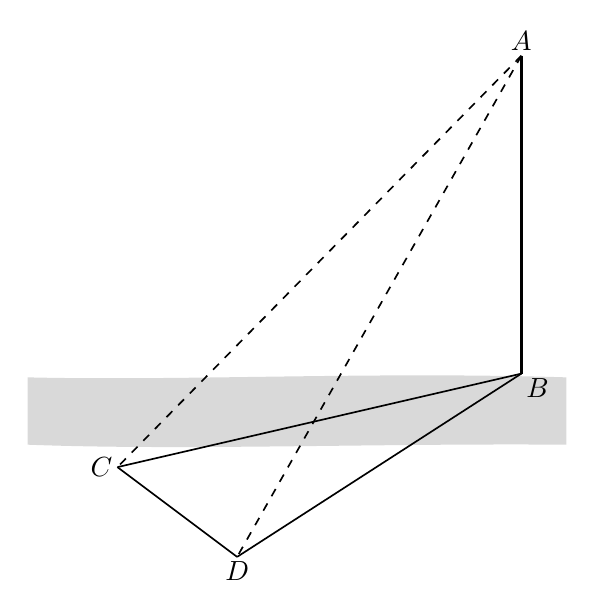
\begin{tikzpicture}[scale=0.95, semithick,
  every node/.style={inner sep=1.5pt}]

  \coordinate (B) at (4.0,0.95);
  \coordinate (A) at (4.0,5.2);
  \coordinate (C) at (-1.4,-0.3);
  \coordinate (D) at (0.2,-1.5);

  % 河面（近岸与对岸之间的灰色带）
  \fill[gray!30]
    (-2.6,0.0) .. controls (-0.5,-0.08) and (2.0,0.02) .. (4.6,0.0)
    -- (4.6,0.9) .. controls (2.0,0.98) and (-0.5,0.85) .. (-2.6,0.9) -- cycle;

  % 塔
  \draw[line width=1.1pt] (A) -- (B);
  \node[above] at (A) {$A$};
  \node[below right] at (B) {$B$};

  % 水平基线与视线
  \draw (C) -- (D);
  \draw (B) -- (C);
  \draw (B) -- (D);
  \draw[dashed] (A) -- (C);
  \draw[dashed] (A) -- (D);

  \node[left] at (C) {$C$};
  \node[below] at (D) {$D$};
\end{tikzpicture}
\end{center}
\nopagebreak[4]
\Needspace{4\baselineskip}
\textbf{解析}

\Needspace{5\baselineskip}
在 $\triangle BCD$ 中，

\nopagebreak[4]
\[\angle CBD=180^\circ-\alpha-\beta.\]

\Needspace{5\baselineskip}
由正弦定理，

\nopagebreak[4]
\[\frac{BC}{\sin\beta}=\frac{s}{\sin(\alpha+\beta)},\]

\Needspace{5\baselineskip}
故

\nopagebreak[4]
\[BC=\frac{s\sin\beta}{\sin(\alpha+\beta)}.\]

\Needspace{5\baselineskip}
在 $\mathrm{Rt}\triangle ABC$ 中，$AB\perp$ 水平面，$\angle ACB=\theta$，故

\nopagebreak[4]
\[AB=BC\tan\theta=\frac{s\sin\beta\tan\theta}{\sin(\alpha+\beta)}.\]

（判断要点：先在水平面内的 $\triangle BCD$ 中用正弦定理求 $BC$，再在竖直直角三角形中用仰角正切求塔高。）

\gkanswer{答案：$AB=\dfrac{s\sin\beta\tan\theta}{\sin(\alpha+\beta)}$。}

\end{answer}
\begin{answer}
\gksolhead{18}{}

\textbf{题目}：

如图，$A$，$B$，$C$，$D$ 为空间四点。在 $\triangle ABC$ 中，$AB=2$，$AC=BC=\sqrt2$，等边三角形 $ADB$ 以 $AB$ 为轴运动。

（1）当平面 $ADB\perp$ 平面 $ABC$ 时，求 $CD$；

（2）当 $\triangle ADB$ 转动时，是否总有 $AB\perp CD$？证明你的结论。
\nopagebreak[4]
\begin{center}% 2007 年新课标卷文科第 18 题：空间四点 A、B、C、D，△ADB 以 AB 为轴转动。
%   D 为顶点，A、B 为轴的两端，C 为底面点；AB 被面 DBC 遮挡，画虚线。
% 来源 PDF：gaokaomath-src/普通高考/2007/2007新课标文(海南,宁夏).pdf
% SHA-256：920ab7ed3244ae8c738e34446fd4135b3a5c50c71fb5e03c3eba0f8a7cbcf804
% 原页：2007新课标文(海南,宁夏).pdf 第 1 页（A3 三栏）第 3 栏，书页码 395。
% 重绘依据：按原页 D、A、B、C 的相对位置与虚实线重绘。
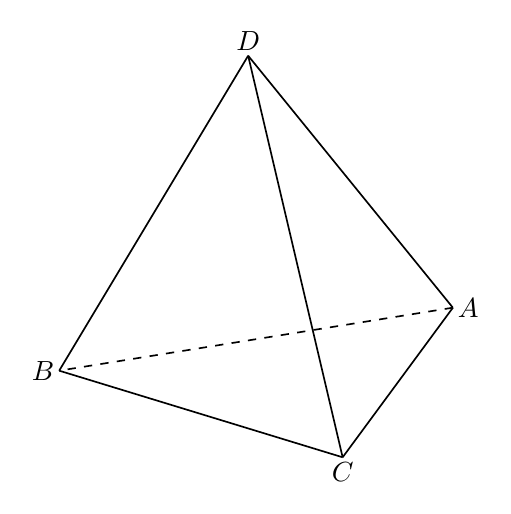
\begin{tikzpicture}[scale=1.0, semithick,
  every node/.style={inner sep=1.5pt}]

  \coordinate (D) at (0,4.0);
  \coordinate (A) at (2.6,0.8);
  \coordinate (B) at (-2.4,0.0);
  \coordinate (C) at (1.2,-1.1);

  \draw (D) -- (A);
  \draw (D) -- (B);
  \draw (D) -- (C);
  \draw (A) -- (C);
  \draw (B) -- (C);
  \draw[dashed] (A) -- (B);

  \node[above] at (D) {$D$};
  \node[right] at (A) {$A$};
  \node[left] at (B) {$B$};
  \node[below] at (C) {$C$};
\end{tikzpicture}
\end{center}
\nopagebreak[4]
\Needspace{4\baselineskip}
\textbf{解析}

（1）设 $M$ 为 $AB$ 中点。

\Needspace{5\baselineskip}
在 $\triangle ABC$ 中，$AC=BC=\sqrt2$，$AB=2$，故

\nopagebreak[4]
\[AC^2+BC^2=2+2=4=AB^2,\]

\Needspace{5\baselineskip}
所以 $\angle ACB=90^\circ$，$CM$ 为斜边中线：

\nopagebreak[4]
\[CM=\frac{AB}{2}=1.\]

\Needspace{5\baselineskip}
等边三角形 $ADB$ 的边长为 $2$，故

\nopagebreak[4]
\[DM=\frac{\sqrt3}{2}\times2=\sqrt3.\]

因为 $AC=BC$，$M$ 为 $AB$ 中点，所以 $CM\perp AB$；同理 $DM\perp AB$。

\Needspace{5\baselineskip}
当平面 $ADB\perp$ 平面 $ABC$ 时，$CM$ 与 $DM$ 分别是两平面内垂直于交线 $AB$ 的直线，故 $CM\perp DM$。于是

\nopagebreak[4]
\[CD=\sqrt{CM^2+DM^2}=\sqrt{1+3}=2.\]

（2）总有 $AB\perp CD$。

证明：由 $AC=BC$ 且 $M$ 为 $AB$ 中点，得 $CM\perp AB$；由 $AD=BD$ 且 $M$ 为 $AB$ 中点，得 $DM\perp AB$。

\Needspace{5\baselineskip}
$CM$ 与 $DM$ 是平面 $CDM$ 内两条相交直线，且都垂直于 $AB$，所以

\nopagebreak[4]
\[AB\perp\text{\text{平面} }CDM.\]

\Needspace{5\baselineskip}
又 $CD\subset$ 平面 $CDM$，故

\nopagebreak[4]
\[AB\perp CD.\]

这一结论与 $\triangle ADB$ 绕 $AB$ 转到什么位置无关。

（判断要点：第（1）问先由勾股定理逆定理得 $\angle ACB=90^\circ$，再用面面垂直时“垂直于交线的两条直线互相垂直”；第（2）问关键是 $C$ 与 $D$ 都在 $AB$ 的垂直平分面内，故 $CD$ 在该平面内，$AB$ 垂直于整个平面。）

\gkanswer{答案：（1）$CD=2$；（2）总有 $AB\perp CD$。}

\end{answer}
\begin{answer}
\gksolhead{19}{}

\textbf{题目}：

设函数 $f(x)=\ln(2x+3)+x^2$。

（1）讨论 $f(x)$ 的单调性；

（2）求 $f(x)$ 在区间 $\left[-\dfrac34,\dfrac14\right]$ 的最大值和最小值。

\Needspace{4\baselineskip}
\textbf{解析}

\Needspace{5\baselineskip}
（1）定义域为 $x>-\dfrac32$。

\nopagebreak[4]
\[f'(x)=\frac2{2x+3}+2x=\frac{2+2x(2x+3)}{2x+3}=\frac{4x^2+6x+2}{2x+3}=\frac{2(2x+1)(x+1)}{2x+3}.\]

分母恒正，分子零点为 $x=-1$ 与 $x=-\dfrac12$。

\begin{itemize}
\item $-\dfrac32<x<-1$ 时，$(2x+1)<0$，$(x+1)<0$，乘积为正，$f'(x)>0$，$f$ 递增；
\item $-1<x<-\dfrac12$ 时，$(2x+1)<0$，$(x+1)>0$，乘积为负，$f'(x)<0$，$f$ 递减；
\item $x>-\dfrac12$ 时，两个因子都为正，$f'(x)>0$，$f$ 递增。
\end{itemize}

故增区间为 $\left(-\dfrac32,-1\right)$ 与 $\left(-\dfrac12,+\infty\right)$，减区间为 $\left(-1,-\dfrac12\right)$。

\Needspace{5\baselineskip}
（2）在 $\left[-\dfrac34,\dfrac14\right]$ 上，$-\dfrac12$ 是极小值点，故最小值

\nopagebreak[4]
\[f\left(-\frac12\right)=\ln(2\times(-\tfrac12)+3)+\frac14=\ln2+\frac14.\]

\Needspace{5\baselineskip}
最大值在端点取得。计算：

\nopagebreak[4]
\[f\left(-\frac34\right)=\ln\left(2\times(-\tfrac34)+3\right)+\frac9{16}=\ln\frac32+\frac9{16},\]

\nopagebreak[4]
\[f\left(\frac14\right)=\ln\left(2\times\frac14+3\right)+\frac1{16}=\ln\frac72+\frac1{16}.\]

\Needspace{5\baselineskip}
比较：

\nopagebreak[4]
\[f\left(\frac14\right)-f\left(-\frac34\right)=\ln\frac73+\frac1{16}-\frac9{16}=\ln\frac73-\frac12.\]

\Needspace{5\baselineskip}
因为 $\dfrac73>\sqrt{\mathrm e}\approx1.648$，所以 $\ln\dfrac73>\dfrac12$，故最大值为

\nopagebreak[4]
\[\ln\frac72+\frac1{16}.\]

（判断要点：先由 $f'$ 的符号确定单调区间；在闭区间上最小值在极小值点，最大值要比较两个端点，不能默认右端点更大。）

\gkanswer{答案：（1）增区间 $\left(-\dfrac32,-1\right)$，$\left(-\dfrac12,+\infty\right)$，减区间 $\left(-1,-\dfrac12\right)$；（2）最大值 $\ln\dfrac72+\dfrac1{16}$，最小值 $\ln2+\dfrac14$。}

\end{answer}
\begin{answer}
\gksolhead{20}{}

\textbf{题目}：

设有关于 $x$ 的一元二次方程 $x^2+2ax+b^2=0$。

（1）若 $a$ 是从 $0$，$1$，$2$，$3$ 四个数中任取的一个数，$b$ 是从 $0$，$1$，$2$ 三个数中任取的一个数，求上述方程有实根的概率；

（2）若 $a$ 是从区间 $[0,3]$ 任取的一个数，$b$ 是从区间 $[0,2]$ 任取的一个数，求上述方程有实根的概率。

\Needspace{4\baselineskip}
\textbf{解析}

\Needspace{5\baselineskip}
（1）$a$ 有 $4$ 种取法，$b$ 有 $3$ 种取法，基本事件总数为

\nopagebreak[4]
\[4\times3=12.\]

\Needspace{5\baselineskip}
方程有实根等价于

\nopagebreak[4]
\[\Delta=(2a)^2-4b^2=4(a^2-b^2)\geqslant0\ \Rightarrow\ a\geqslant b.\]

逐一计数：

\begin{itemize}
\item $a=0$：$b=0$，共 $1$ 个；
\item $a=1$：$b=0,1$，共 $2$ 个；
\item $a=2$：$b=0,1,2$，共 $3$ 个；
\item $a=3$：$b=0,1,2$，共 $3$ 个。
\end{itemize}

\Needspace{5\baselineskip}
有利事件共

\nopagebreak[4]
\[1+2+3+3=9,\]

\Needspace{5\baselineskip}
故概率

\nopagebreak[4]
\[P=\frac9{12}=\frac34.\]

\Needspace{5\baselineskip}
（2）$a\in[0,3]$，$b\in[0,2]$，样本空间是面积为

\nopagebreak[4]
\[3\times2=6\]

的矩形。

\Needspace{5\baselineskip}
有利区域为 $a\geqslant b$。其补集为 $a<b$，即 $0\leqslant b\leqslant2$ 且 $0\leqslant a<b$，面积为

\nopagebreak[4]
\[\int_0^2 b\,\mathrm db=\frac12\times2^2=2.\]

\Needspace{5\baselineskip}
故有利区域面积

\nopagebreak[4]
\[6-2=4,\]

\Needspace{5\baselineskip}
概率

\nopagebreak[4]
\[P=\frac46=\frac23.\]

（判断要点：第（1）问是古典概型，逐个数对；第（2）问是几何概型，画矩形与直线 $a=b$，用面积比。）

\gkanswer{答案：（1）$\dfrac34$；（2）$\dfrac23$。}

\end{answer}
\begin{answer}
\gksolhead{21}{}

\textbf{题目}：

在平面直角坐标系 $xOy$ 中，已知圆 $x^2+y^2-12x+32=0$ 的圆心为 $Q$，过点 $P(0,2)$ 且斜率为 $k$ 的直线与圆 $Q$ 相交于不同的交点 $A$，$B$。

（1）求 $k$ 的取值范围；

（2）是否存在常数 $k$，使得向量 $\overrightarrow{OA}+\overrightarrow{OB}$ 与 $\overrightarrow{PQ}$ 共线？如果存在，求 $k$ 值；如果不存在，请说明理由。

\Needspace{4\baselineskip}
\textbf{解析}

\Needspace{5\baselineskip}
（1）圆方程配方：

\nopagebreak[4]
\[x^2+y^2-12x+32=0\ \Rightarrow\ (x-6)^2+y^2=4.\]

圆心 $Q(6,0)$，半径 $2$。

\Needspace{5\baselineskip}
直线过 $P(0,2)$、斜率为 $k$：

\nopagebreak[4]
\[y=kx+2,\]

\Needspace{5\baselineskip}
即

\nopagebreak[4]
\[kx-y+2=0.\]

\Needspace{5\baselineskip}
直线与圆有两个不同交点，需圆心到直线距离小于半径：

\nopagebreak[4]
\[\frac{|6k-0+2|}{\sqrt{k^2+1}}<2.\]

\Needspace{5\baselineskip}
平方：

\nopagebreak[4]
\[(6k+2)^2<4(k^2+1),\]

\nopagebreak[4]
\[36k^2+24k+4<4k^2+4,\]

\nopagebreak[4]
\[32k^2+24k<0,\]

\nopagebreak[4]
\[8k(4k+3)<0.\]

\Needspace{5\baselineskip}
故

\nopagebreak[4]
\[-\frac34<k<0.\]

\Needspace{5\baselineskip}
（2）设 $A(x_1,y_1)$，$B(x_2,y_2)$。把 $y=kx+2$ 代入圆方程：

\nopagebreak[4]
\[(x-6)^2+(kx+2)^2=4,\]

\Needspace{5\baselineskip}
展开：

\nopagebreak[4]
\[x^2-12x+36+k^2x^2+4kx+4=4,\]

\Needspace{5\baselineskip}
即

\nopagebreak[4]
\[(1+k^2)x^2+(4k-12)x+36=0.\]

\Needspace{5\baselineskip}
由韦达定理，

\nopagebreak[4]
\[x_1+x_2=\frac{12-4k}{1+k^2}.\]

\Needspace{5\baselineskip}
又

\nopagebreak[4]
\[y_1+y_2=k(x_1+x_2)+4=\frac{k(12-4k)}{1+k^2}+4=\frac{12k-4k^2+4+4k^2}{1+k^2}=\frac{12k+4}{1+k^2}.\]

\Needspace{5\baselineskip}
故

\nopagebreak[4]
\[\overrightarrow{OA}+\overrightarrow{OB}=\left(\frac{12-4k}{1+k^2},\frac{12k+4}{1+k^2}\right).\]

\Needspace{5\baselineskip}
又

\nopagebreak[4]
\[\overrightarrow{PQ}=Q-P=(6,-2).\]

\Needspace{5\baselineskip}
若两向量共线，则

\nopagebreak[4]
\[\frac{12-4k}{1+k^2}\cdot(-2)-\frac{12k+4}{1+k^2}\cdot6=0.\]

\Needspace{5\baselineskip}
化简：

\nopagebreak[4]
\[-2(12-4k)-6(12k+4)=0,\]

\nopagebreak[4]
\[-24+8k-72k-24=0,\]

\nopagebreak[4]
\[-48-64k=0,\]

\nopagebreak[4]
\[k=-\frac34.\]

但 $k=-\dfrac34$ 不在（1）的范围内（此时直线与圆相切，只有一个交点），故不存在这样的常数 $k$。

（判断要点：第（1）问用圆心到直线距离小于半径；第（2）问用韦达定理求中点坐标，再写共线条件，最后必须回代检验 $k$ 是否在（1）的范围内。）

\gkanswer{答案：（1）$-\dfrac34<k<0$；（2）不存在。}

\end{answer}
\begin{answer}
\gksolhead{22}{}

\textbf{题目}：

如图，已知 $AP$ 是 $\odot O$ 的切线，$P$ 为切点，$AC$ 是 $\odot O$ 的割线，与 $\odot O$ 交于 $B$，$C$ 两点，圆心 $O$ 在 $\angle PAC$ 的内部，点 $M$ 是 $BC$ 的中点。

（1）证明 $A$，$P$，$O$，$M$ 四点共圆；

（2）求 $\angle OAM+\angle APM$ 的大小。
\nopagebreak[4]
\begin{center}% 2007 年新课标卷文科第 22 题：圆的切线 AP、割线 ABC、弦 BC 中点 M。
%   圆 O 半径 2，A(-4,0)，切点 P=(-1,√3)；
%   割线 ABC 从 A 出发，B、C 为与圆的交点，M 为 BC 中点。
% 来源 PDF：gaokaomath-src/普通高考/2007/2007新课标文(海南,宁夏).pdf
% SHA-256：c8ee1632ac3a7a28aab1150f047a2e1c74398ca2944701e9165237897ae724e2
% 原页：2007新课标文(海南,宁夏).pdf 第 2 页（A3 三栏）第 3 栏，书页码 394。
% 重绘依据：按原页点、线与圆的位置重绘；A-O 与 P-M 为题目用到的辅助线。
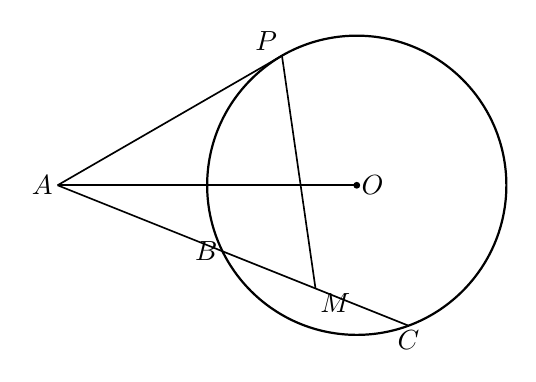
\begin{tikzpicture}[scale=0.95, semithick,
  every node/.style={inner sep=1.5pt}]

  \coordinate (O) at (0,0);
  \coordinate (A) at (-4,0);
  \coordinate (P) at (-1,1.732);
  \coordinate (B) at (-1.795,-0.882);
  \coordinate (C) at (0.692,-1.877);
  \coordinate (M) at (-0.5515,-1.3795);

  \draw[thick] (O) circle (2);
  \fill (O) circle (1.3pt);

  % 切线、割线与辅助线
  \draw (A) -- (P);
  \draw (A) -- (C);
  \draw (A) -- (O);
  \draw (P) -- (M);

  \node[left] at (A) {$A$};
  \node[above left] at (P) {$P$};
  \node[right] at (O) {$O$};
  \node[left] at (B) {$B$};
  \node[below] at (C) {$C$};
  \node[below right] at (M) {$M$};
\end{tikzpicture}
\end{center}
\nopagebreak[4]
\Needspace{4\baselineskip}
\textbf{解析}

\Needspace{5\baselineskip}
（1）$AP$ 是切线，$P$ 为切点，故

\nopagebreak[4]
\[OP\perp AP\ \Rightarrow\ \angle OPA=90^\circ.\]

\Needspace{5\baselineskip}
$M$ 是弦 $BC$ 的中点，故

\nopagebreak[4]
\[OM\perp BC.\]

\Needspace{5\baselineskip}
又 $A$，$B$，$M$，$C$ 共线，所以 $OM\perp AM$，即

\nopagebreak[4]
\[\angle OMA=90^\circ.\]

于是 $P$ 与 $M$ 都在以 $AO$ 为直径的圆上，故 $A$，$P$，$O$，$M$ 四点共圆。

\Needspace{5\baselineskip}
（2）由（1）四点共圆，$\angle APM$ 与 $\angle AOM$ 都是弧 $AM$ 所对的圆周角，故

\nopagebreak[4]
\[\angle APM=\angle AOM.\]

\Needspace{5\baselineskip}
于是

\nopagebreak[4]
\[\angle OAM+\angle APM=\angle OAM+\angle AOM.\]

\Needspace{5\baselineskip}
在 $\triangle AOM$ 中，$\angle AMO=90^\circ$，故

\nopagebreak[4]
\[\angle OAM+\angle AOM=90^\circ.\]

\Needspace{5\baselineskip}
所以

\nopagebreak[4]
\[\angle OAM+\angle APM=90^\circ.\]

（判断要点：四点共圆用“以 $AO$ 为直径的圆”；第（2）问用同弧所对圆周角相等，把 $\angle APM$ 换成 $\angle AOM$。）

\gkanswer{答案：（1）证明见解析；（2）$90^\circ$。}

\end{answer}
\begin{answer}
\gksolhead{23}{}

\textbf{题目}：

$\odot O_1$ 和 $\odot O_2$ 的极坐标方程分别为 $\rho=4\cos\theta$，$\rho=-4\sin\theta$。

（1）把 $\odot O_1$ 和 $\odot O_2$ 的极坐标方程化为直角坐标方程；

（2）求经过 $\odot O_1$，$\odot O_2$ 交点的直线的直角坐标方程。

\Needspace{4\baselineskip}
\textbf{解析}

\Needspace{5\baselineskip}
（1）由 $\rho=4\cos\theta$，两边乘 $\rho$：

\nopagebreak[4]
\[\rho^2=4\rho\cos\theta\ \Rightarrow\ x^2+y^2=4x\ \Rightarrow\ (x-2)^2+y^2=4.\]

\Needspace{5\baselineskip}
由 $\rho=-4\sin\theta$，两边乘 $\rho$：

\nopagebreak[4]
\[\rho^2=-4\rho\sin\theta\ \Rightarrow\ x^2+y^2=-4y\ \Rightarrow\ x^2+(y+2)^2=4.\]

\Needspace{5\baselineskip}
（2）两圆方程分别为

\nopagebreak[4]
\[x^2+y^2-4x=0,\qquad x^2+y^2+4y=0.\]

\Needspace{5\baselineskip}
相减：

\nopagebreak[4]
\[-4x-4y=0\ \Rightarrow\ x+y=0.\]

这就是经过两圆交点的直线（公共弦）的直角坐标方程。

（判断要点：极坐标化直角坐标时两边乘 $\rho$ 是关键；两圆方程相减直接得公共弦。）

\gkanswer{答案：（1）$(x-2)^2+y^2=4$，$x^2+(y+2)^2=4$；（2）$x+y=0$。}

\end{answer}
\begin{answer}
\gksolhead{24}{}

\textbf{题目}：

设函数 $f(x)=|2x+1|-|x-4|$。

（1）解不等式 $f(x)>2$；

（2）求函数 $y=f(x)$ 的最小值。

\Needspace{4\baselineskip}
\textbf{解析}

\Needspace{5\baselineskip}
零点为 $x=-\dfrac12$ 与 $x=4$，分三段：

\nopagebreak[4]
\[f(x)=\begin{cases}-x-5,&x<-\dfrac12,\\ 3x-3,&-\dfrac12\leqslant x<4,\\ x+5,&x\geqslant4.\end{cases}\]

（1）解 $f(x)>2$：

\begin{itemize}
\item $x<-\dfrac12$：$-x-5>2$，得 $x<-7$；
\item $-\dfrac12\leqslant x<4$：$3x-3>2$，得 $x>\dfrac53$，即 $\dfrac53<x<4$；
\item $x\geqslant4$：$x+5>2$ 恒成立，即 $x\geqslant4$。
\end{itemize}

\Needspace{5\baselineskip}
合并得

\nopagebreak[4]
\[x<-7\ \text{\text{或}}\ x>\frac53.\]

（2）各段最小值：

\begin{itemize}
\item $x<-\dfrac12$：$-x-5>-\dfrac92$；
\item $-\dfrac12\leqslant x<4$：$3x-3\geqslant-\dfrac92$；
\item $x\geqslant4$：$x+5\geqslant9$。
\end{itemize}

\Needspace{5\baselineskip}
故最小值为

\nopagebreak[4]
\[f\left(-\frac12\right)=-\frac92.\]

（判断要点：分段去绝对值时 $|x-4|=4-x$（当 $x<4$）；最小值在分界点 $x=-\dfrac12$ 取到。）

\gkanswer{答案：（1）$x<-7$ 或 $x>\dfrac53$；（2）$-\dfrac92$。}

\end{answer}